\documentclass[11pt, addpoints, answers]{exam}

\usepackage{amsmath, amssymb, amsthm}
\usepackage{xcolor}
\usepackage{graphicx}
\usepackage{graphics}
\usepackage{enumerate}


\usepackage{tikz}
\usepackage{tikz-qtree}
\usetikzlibrary{graphs}
\usetikzlibrary{arrows.meta}
\usepackage{listings}   
\usepackage{caption}
\makeatletter
\makeatother


\usepackage{algorithm}
\usepackage{algorithmic}




% For inserting code snippets.
\usepackage{listings}
\lstset{
	columns = fixed,
	basewidth = {0.5em},
	breaklines = true,
	backgroundcolor = \color{white},
	keywordstyle = \color[RGB]{40, 40, 255},
	numberstyle = \footnotesize\color{darkgray},
	commentstyle = \ttfamily\color{violet},
	basicstyle = \ttfamily,
	stringstyle = \ttfamily\color[RGB]{128, 0, 0},
	showstringspaces = false,
	language = {[11]C++},
	escapechar = \@
}
\lstnewenvironment{cpp}[1][]{\lstset{language = {[11]C++}, #1}}{}

\usepackage{tikz}

% headers, footers, titles
\newcommand{\CourseName}{CS101 Algorithms and Data Structures}
\newcommand{\HomeworkNO}{Homework 7}
\newcommand{\DueDate}{Due date: 23:59, November 13th, 2022}

\pagestyle{headandfoot}
\runningheadrule
\runningheader{\CourseName}{\HomeworkNO}{\DueDate}
\runningfooter{}{\thepage}{}

\title{
	\CourseName\\
	Fall 2022\\
	\HomeworkNO
}
\author{}
\date{\DueDate}

% formats of questions, choices, points, etc.
\qformat{\bf\thequestion. (\totalpoints\ points) \thequestiontitle\hfill}
\pointname{'}
\CorrectChoiceEmphasis{\bf\color{blue}}
\SolutionEmphasis{\color{blue}}

% We frequently use this font.
\newcommand{\ttt}{\texttt}

\begin{document}

\maketitle

\begin{enumerate}
	\item Please write your solutions in English.
	\item Submit your solutions to gradescope.com.
	\item Set your FULL name to your Chinese name and your STUDENT ID correctly in Account Settings.
	\item If you want to submit a handwritten version, scan it clearly. \ttt{CamScanner} is recommended.
	\item When submitting, match your solutions to the problems correctly.
	\item No late submission will be accepted.
	\item Violations to any of the above may result in zero points.
\end{enumerate}

\begin{questions}

	\titledquestion{Multiple Choices}

Each question has \textbf{one or more} correct answer(s). Select all the correct answer(s). For each question, you will get 0 points if you select one or more wrong answers, but you will get 1 point if you select a non-empty subset of the correct answers.

Write your answers in the following table.

%%%%%%%%%%%%%%%%%%%%%%%%%%%%%%%%%%%%%%%%%%%%%%%%%%%%%%%%%%%%%%%%%%%%%%%%%%%
% Note: The `LaTeX' way to answer a multiple-choices question is to replace `\choice'
% with `\choice', as what you did in the previous questions. However, there are 
% still many students who would like to handwrite their homework. To make TA's work 
% easier, you have to fill your selected choices in the table below, no matter whether 
% you use LaTeX or not.
%%%%%%%%%%%%%%%%%%%%%%%%%%%%%%%%%%%%%%%%%%%%%%%%%%%%%%%%%%%%%%%%%%%%%%%%%%%

\begin{table}[htbp]
	\centering
	\begin{tabular}{|p{1.7cm}|p{1.7cm}|p{1.7cm}|p{1.7cm}|p{1.7cm}|p{1.7cm}|p{1.7cm}|p{1.7cm}|p{1.7cm}|}
		\hline
		(a) & (b) & (c) & (d) & (e) & (f) \\
		\hline
		%%%%%%%%%%%%%%%%%%%%%%%%%%%%%%%%%%%%%%%%%%%%%%%%%%%%%%%%%%
		% YOUR ANSWER HERE.
		    &     &     &     &     &     \\
		%%%%%%%%%%%%%%%%%%%%%%%%%%%%%%%%%%%%%%%%%%%%%%%%%%%%%%%%%%
		\hline
	\end{tabular}
\end{table}

\begin{parts}
    \part[2] A planar graph is a graph which can be embedded in a plane i.e. you can find a way to put all vertices on the plane where the edges will not intersect with each other. Which of the statement(s) is/are correct?
    \begin{choices}
        \choice $\forall n\leq 5, K_n$ is planar. $K_n$ means the complete graph with $n$ vertices.
        \choice $K_6$ is not planar.
        \choice DAGs are planar.
        \choice A tree is planar.
        \choice Bipartite graphs are planar.
    \end{choices}

    \part[2] Given a graph $G=(V,E)$, $w(e)$ indicates the weight of edge $e$. Which of the statement(s) is/are correct?
    \begin{choices}
        \choice Both Kruskal's and Prim's algorithms can correctly find the MST even when $\exists e, w(e)<0$.
        \choice Suppose $G$ is connected and $|E| = \omega(|V|)$, $G$ has a unique MST if and only if $\forall e,e'\in E, w(e) = w(e') \Leftrightarrow e = e'$ i.e. weights of edges are distinct.
        \choice Suppose $G' = (V,E)$ is the same graph as $G$ with different weight function $v(e)$. If they share a same MST $T$, then $T$ is also the MST of $G$ with weights $u(e) = w(e) + v(e)$.
        \choice If $G$ contains multi-edges i.e. $G$ is not simple, then Kruskal's algorithm will fail but Prim's won't fail when finding MST.
    \end{choices}

	\part[2] Given a graph $G=(V,E)$, which of the following is(are) correct? 
	\begin{choices}
		\choice If $G$ is a complete graph with $4$ vertices, then the number of spanning trees of $G$ is $16$.
		\choice After Kruskal's algorithm, we choose $m$ edges, then the number of connected components of $G$ is $|V|-m$.
		\choice If $G$ is stored in adjacency matrix, then the total time complexity of Kruskal's algorithm can reach $\Theta(|V|^2+|E|\log|E|)$.
        \choice Suppose $G$ is connected and $|V| = |E|$, the maximum number of spanning trees of $G$ can reach $\Theta(|V|)$.
	\end{choices}
    
    \part[2] Let $G$ be a weighted undirected graph with positive weights where edge $e$ has weight $w_e\in \mathbb{R}^+$ for all $e \in E$. A new graph $G'$, which is a copy of $G$, and the weight of each edge $e$ in $G'$ is transformed using a function $f(w_e)$. Which of the following statements is/are true?

    \begin{choices} 
        \choice If $f(w_e) = w_e^2$, then any MST in $G$ is also an MST in $G'$.
        \choice If $f(w_e) = 2^{w_e}$, then any MST in $G$ is also an MST in $G'$.
        \choice If $f(w_e) = \frac1 {w_e}$, then any MST in $G$ is also an MST in $G'$.
        \choice If $f(w_e) = \log (w_e)$, then any MST in $G$ is also an MST in $G'$.
    \end{choices}

	\part[2] What is the number of spanning trees of following graph?

    \begin{center}
    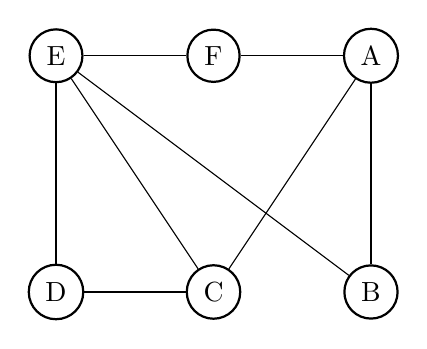
\begin{tikzpicture}
        \begin{scope}[every node/.style = {circle, thick, draw}]
            \node (A) at (2,0) {A};
            \node (B) at (2, -3) {B};
            \node (C) at (0, -3) {C};
            \node (D) at (-2, -3) {D};
            \node (E) at (-2, 0) {E};
            \node (F) at (0,0) {F};
        \end{scope}
        \begin{scope}
            \path[-] (E) edge (D);
            \path[-] (E) edge (C);
            \path[-] (E) edge (B);
            \path[-] (C) edge (D);
            \path[-] (B) edge (A);
            \path[-] (A) edge (C);
            \path[-] (A) edge (F);
            \path[-] (E) edge (F);
        \end{scope}
    \end{tikzpicture}
    \end{center}
	\begin{choices}
		\choice 32
		\choice 34
		\choice 36
		\choice 38
	\end{choices}

        \part[2] Which of the following statements are true for MST(Minimum Spanning Tree)?
        \begin{choices}
            \choice Suppose $G$ has multiple MSTs. For each minimum spanning tree $T$ of a graph $G$, there is a way to sort the edges of $G$ in Kruskal’s algorithm so that the algorithm returns $T$.
            \choice Prim's algorithm is a divide-and-conquer algorithm because it divides the graph into $S$ and $V-S$ then solve.
            \choice If we use binary heap to optimize Prim's algorithm when choosing the next edge, it will always have a better time complexity than the original algorithm on any graph.
            \choice If we add a new edge $e = (u,v)$ into a graph $G=(V,E)$ with unique MST to get a new graph $G' = (V,E\cup\{e\})$. There is at most $1$ edge difference between the MST of $G$ and $G'$.
        \end{choices}

\end{parts}


	\newpage
	\titledquestion{Graph traversal}
Consider this directed graph starting with \(s\).
\begin{center}
	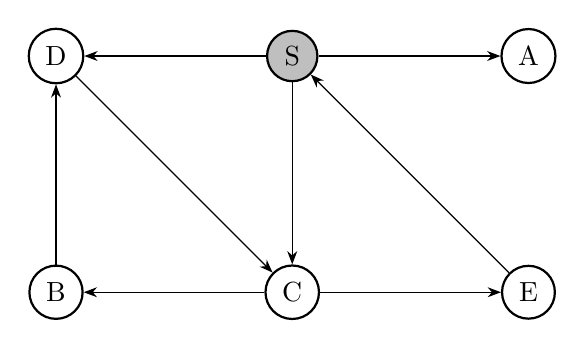
\begin{tikzpicture}
		\begin{scope}[every node/.style = {circle, thick, draw}]
			\node[fill={rgb:black,1;white,3}] (S) at (0,0) {S};
			\node (A) at (3,0) {A};
			\node (B) at (-3, -3) {B};
			\node (C) at (0, -3) {C};
			\node (D) at (-3, 0) {D};
			\node (E) at (3, -3) {E};
		\end{scope}
		\begin{scope}[>={Stealth[black]}]
			\path[->] (S) edge (A);
			\path[->] (S) edge (C);
			\path[->] (S) edge (D);
			\path[->] (B) edge (D);
			\path[->] (C) edge (B);
			\path[->] (C) edge (E);
			\path[->] (D) edge (C);
			\path[->] (E) edge (S);
		\end{scope}
	\end{tikzpicture}

\end{center}

\begin{parts}
	\part[3] Give the adjacency list for the graph. You should write the node in alphabetical order. (If no item, leave it blank).\\
	\[
		\begin{array}{ll}
			adj(S) & = [\fillin[A,C,D]], \\
			adj(A) & = [\fillin[]], \\
			adj(B) & = [\fillin[D]], \\
			adj(C) & = [\fillin[B,E]], \\
			adj(D) & = [\fillin[C]], \\
			adj(E) & = [\fillin[S]], \\
		\end{array}
	\]
	\part[3] Give the visited node order using the above adjacency list for Breadth First Search.
	\begin{solution}
		%\vspace{4ex}
		S,A,C,D,B,E
	\end{solution}
	\part[3] Give the visited node order using the above adjacency list for Depth First Search.
	\begin{solution}
		%\vspace{4ex}
		S,A,C,B,D,E
	\end{solution}
\end{parts}

	\newpage
	\titledquestion{DSU on hand}[2]

\emph{I mean, hands on DSU, perhaps.}\\

Consider performing a series of merge opertions on a disjoint set structure employing union-by-height strategy.
Draw the resulting tree structure.\\
When merging two sets,
break tie by merging the tree whose root label is small into the other tree.

\newcommand{\SET}[1]{\{#1\}}

\begin{enumerate}[{\bf op} 1.]
	\item initialize: $\SET{1}, \SET{2}, \SET{3}, \SET{4}, \SET{5}, \SET{6}, \SET{6}, \SET{7}, \SET{8}$
	\item merge 1,8
	\item merge 2,7
	\item merge 3,6
	\item merge 4,5
	\item merge 1,4
	\item merge 2,3
	\item merge 5,3
\end{enumerate}

\begin{solution}
	% Give tikz-qtree a try!\\
	\vspace{60ex}
	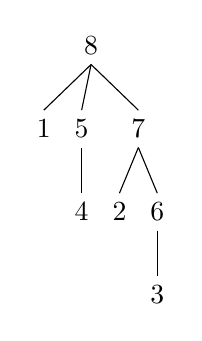
\begin{tikzpicture}
		\Tree [.8
				1
				[
					.5
					4
				]
				[.7
					2
					[
						.6
						3
					]
				]
		]
	\end{tikzpicture}
\end{solution}

	\newpage
	\titledquestion{The highest DSU I've ever seen}

In the following tasks, you can label the nodes by whatever mark you want.
We only care about the tree structure.

\begin{parts}
	\part[2] Plot a union tree of $15$ nodes with minimum height.
	The tree was generated by disjoint-set-union with union-by-height.\\
	\part[2] Plot a union tree of $16$ nodes with maximum height.
	The tree was generated by disjoint-set-union with union-by-height.\\
\end{parts}

\begin{solution}

for (a)\\\\

\begin{enumerate}[(a)]
%		\item Why not tikz?\\
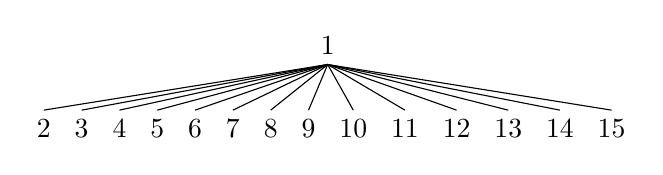
\begin{tikzpicture}
	\Tree [.1
		2 3 4 5 6 7 8 9 10 11 12 13 14 15
	]
\end{tikzpicture}
\end{enumerate}


for (b)\\\\
\begin{enumerate}[(b)]
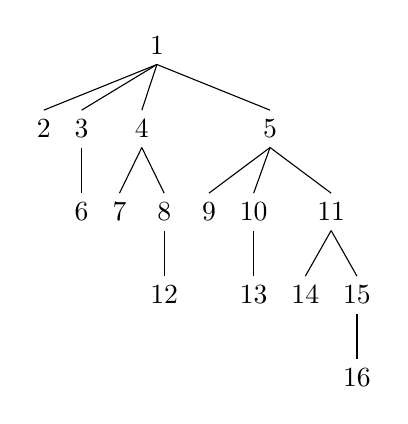
\begin{tikzpicture}
	\Tree [.1
		2
		[
			.3
			6
		]
		[
			.4
			7
			[
				.8
				12
			]
		]
		[
			.5
			9
			[
				.10
				13
			]
			[
				.11
				14
				[
					.15
					16
				]	
			]
		]
	]
\end{tikzpicture}
\end{enumerate}
%Also checkout mathcha.


\vspace{80ex}
\end{solution}



\end{questions}

\end{document}
